\documentclass[pdflatex,sn-mathphys]{sn-jnl}
\jyear{\year}

\usepackage{lipsum}

\raggedbottom

\begin{document}

\title[Modelagem de planta industrial]{Modelagem de planta industrial}

%%=============================================================%%
%% Prefix	-> \pfx{Dr}
%% GivenName	-> \fnm{Joergen W.}
%% Particle	-> \spfx{van der} -> surname prefix
%% FamilyName	-> \sur{Ploeg}
%% Suffix	-> \sfx{IV}
%% NatureName	-> \tanm{Poet Laureate} -> Title after name
%% Degrees	-> \dgr{MSc, PhD}
%% \author*[1,2]{\pfx{Dr} \fnm{Joergen W.} \spfx{van der} \sur{Ploeg} \sfx{IV} \tanm{Poet Laureate} 
%%                 \dgr{MSc, PhD}}\email{iauthor@gmail.com}
%%=============================================================%%

\author*[1]{\fnm{First} \sur{Author}}\email{First@gmail.com}

\author[2,3]{\fnm{Second} \sur{Author}}\email{iiauthor@gmail.com}
\equalcont{These authors contributed equally to this work.}

\author[1,2]{\fnm{Third} \sur{Author}}\email{iiiauthor@gmail.com}
\equalcont{These authors contributed equally to this work.}

\affil*[1]{\orgdiv{PPGEE}, \orgname{UTFPR}, \orgaddress{\street{Via do Conhecimento}, \city{Pato Branco}, \postcode{85503-390}, \state{PR}, \country{Brasil}}}

\affil[2]{\orgdiv{Department}, \orgname{Organization}, \orgaddress{\street{Street}, \city{City}, \postcode{10587}, \state{State}, \country{Country}}}

\affil[3]{\orgdiv{Department}, \orgname{Organization}, \orgaddress{\street{Street}, \city{City}, \postcode{610101}, \state{State}, \country{Country}}}



\abstract{The abstract serves both as a general introduction to the topic and as a brief, non-technical summary of the main results and their implications. Authors are advised to check the author instructions for the journal they are submitting to for word limits and if structural elements like subheadings, citations, or equations are permitted.}

\keywords{keyword1, Keyword2, Keyword3, Keyword4}

%%\pacs[JEL Classification]{D8, H51}

%%\pacs[MSC Classification]{35A01, 65L10, 65L12, 65L20, 65L70}

\maketitle

\section{Modelos projetados}
\subsection{Plantas}
Robôs 1 e 2

TODO: descrição do funcionamento dos robôs

\begin{figure}[H]%
  \centering
  \begin{subfigure}[b]{0.45\textwidth}
      \centering
      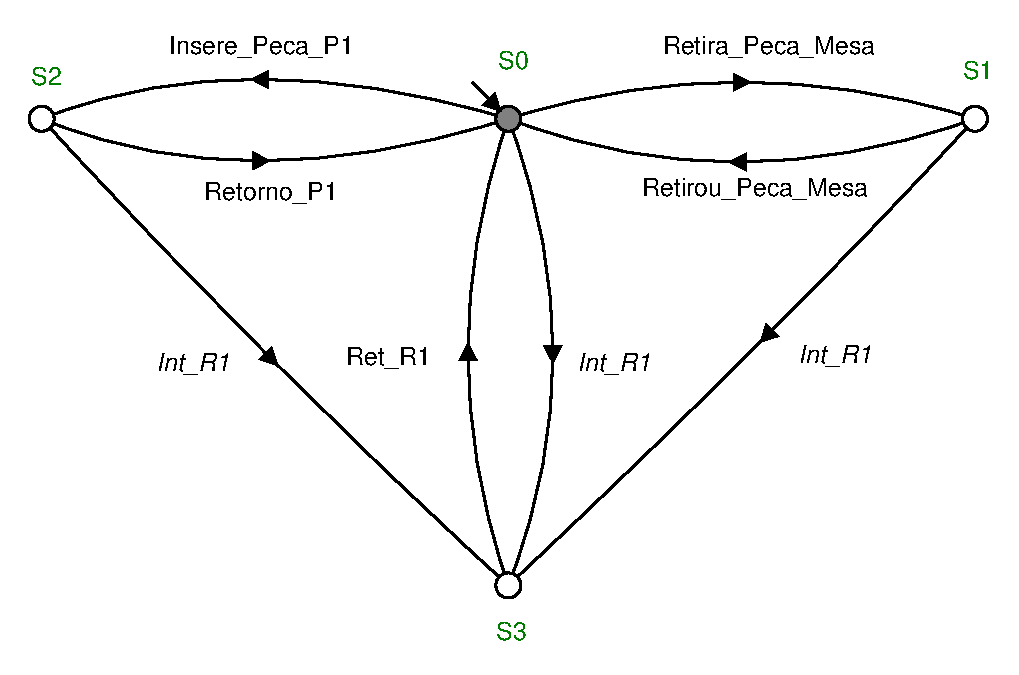
\includegraphics[width=\textwidth]{imagens/Robo_1.eps}
      \caption{Robô 1}
      \label{fig:r1}
  \end{subfigure}
  \hfill
  \begin{subfigure}[b]{0.45\textwidth}
      \centering
      \includegraphics[width=\textwidth]{imagens/Robo_2.eps}
      \caption{Robô 2}
      \label{fig:r2}
  \end{subfigure}
  \caption{Planta Robôs 1 e 2}
  \label{fig:robo12}
\end{figure}

Robôs 3 e 4

TODO: descrição do funcionamento dos robôs

\begin{figure}[H]%
  \centering
  \begin{subfigure}[b]{0.45\textwidth}
      \centering
      \includegraphics[width=\textwidth]{imagens/Robo_3.eps}
      \caption{Robô 3}
      \label{fig:r3}
  \end{subfigure}
  \hfill
  \begin{subfigure}[b]{0.45\textwidth}
      \centering
      \includegraphics[width=\textwidth]{imagens/Robo_4.eps}
      \caption{Robô 4}
      \label{fig:r4}
  \end{subfigure}
  \caption{Planta Robôs 3 e 4}
  \label{fig:robo34}
\end{figure}

Robô 5

TODO: descrição do funcionamento do robô

\begin{figure}[H]%
    \centering
    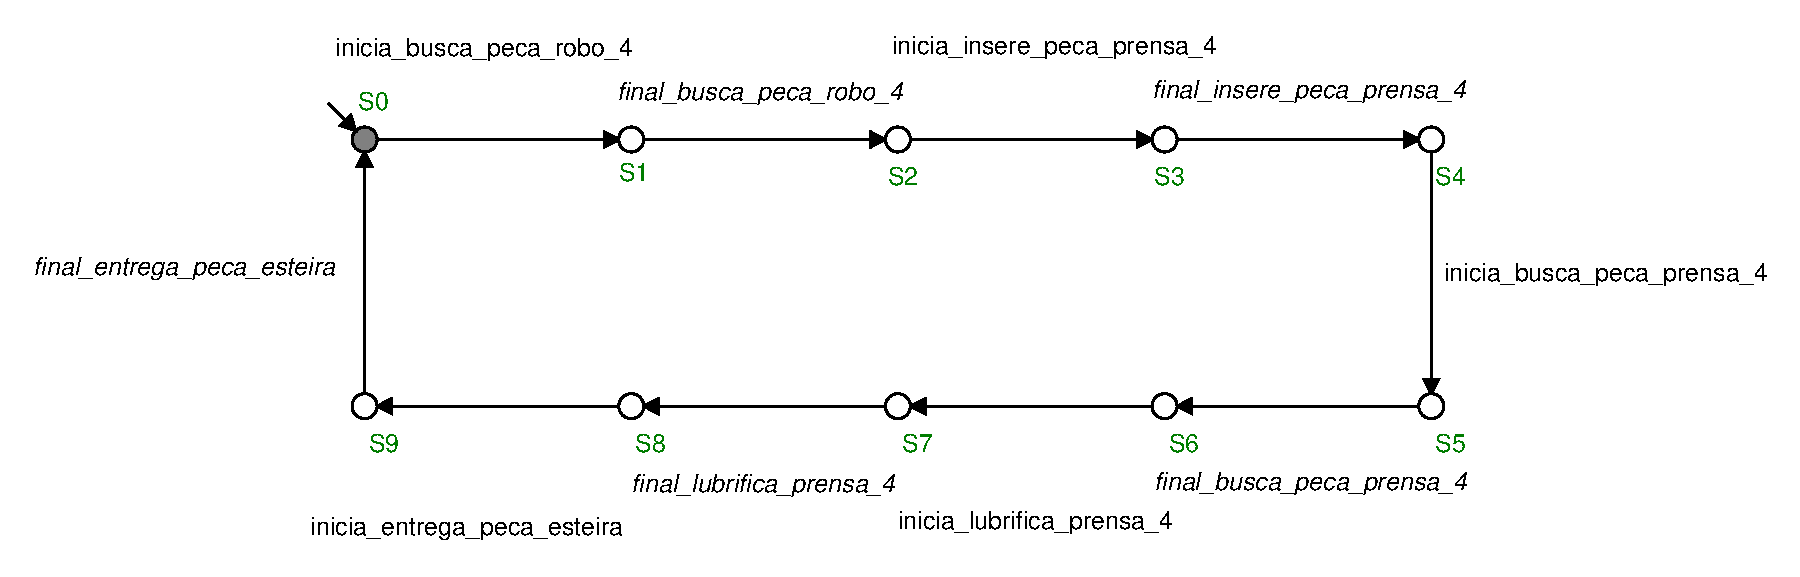
\includegraphics[width=0.9\textwidth]{imagens/robo_5.eps}
    \caption{Planta Robô 3}\label{fig:robo5}
\end{figure}

Todas as prensas têm o mesmo modelo, a seguir apresenta-se o modelo genérico para as prensas.

TODO: descrever funcionamento esperado para uma prensa, talvez.

\begin{figure}[H]%
    \centering
    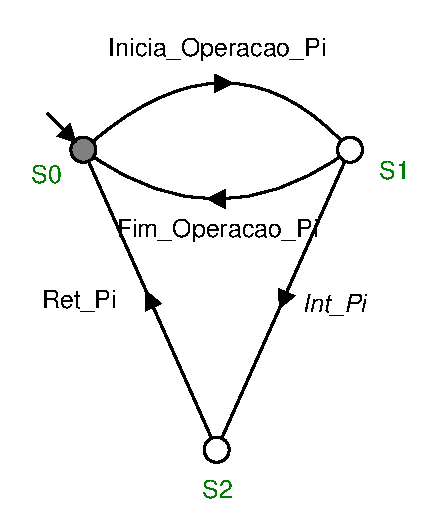
\includegraphics[width=0.6\textwidth]{imagens/Prensa.eps}
    \caption{Planta Prensa}\label{fig:prensa}
\end{figure}

\subsection{Especificações}
A seção a seguir são apresenta as especificações desenvolvidas para cumprir com os requisitos de controle desejados.

A especificação apresentada na Figura \ref{fig:e0} permite ao Robô 1 retirar peças da mesa centralizadora após o sensor detectar existencia de peça sobre a mesa.
Já a especificação apresentada na Figura \ref{fig:e1} limita o Robô 1 a iniciar o processo de inserção na Prensa 1 após ter peça presente na garra.

\begin{figure}[H]%
  \centering
  \begin{subfigure}[b]{0.45\textwidth}
      \centering
      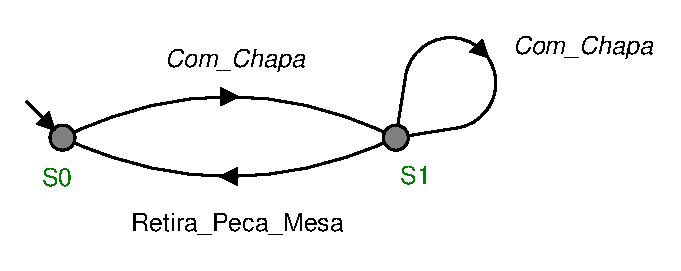
\includegraphics[width=\textwidth]{imagens/E0.eps}
      \caption{E0}
      \label{fig:e0}
  \end{subfigure}
  \hfill
  \begin{subfigure}[b]{0.45\textwidth}
      \centering
      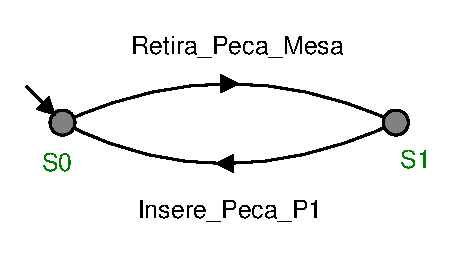
\includegraphics[width=\textwidth]{imagens/E1.eps}
      \caption{E1}
      \label{fig:e1}
  \end{subfigure}
  \caption{Especificações 0 e 1}
  \label{fig:e01}
\end{figure}

A especificação apresentada na Figura \ref{fig:e2} permite que a Prensa 1 inicie a operação após o Robô 1 finalizar a inserção e estar em posição segura.
Já a especificação apresentada na \ref{fig:e3} é o modelo para overflow da Prensa 1 e libera uma nova inserção após a retirada da peça pelo Robô 2.

\begin{figure}[H]%
  \centering
  \begin{subfigure}[b]{0.45\textwidth}
      \centering
      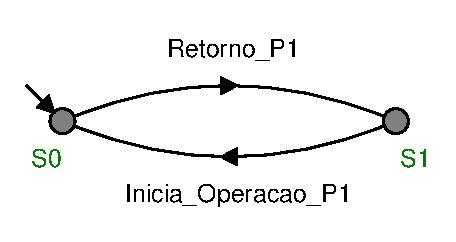
\includegraphics[width=\textwidth]{imagens/E2.eps}
      \caption{E2}
      \label{fig:e2}
  \end{subfigure}
  \hfill
  \begin{subfigure}[b]{0.45\textwidth}
      \centering
      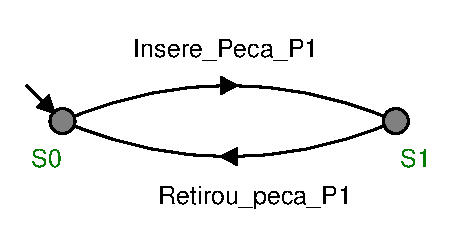
\includegraphics[width=\textwidth]{imagens/E3.eps}
      \caption{E3}
      \label{fig:e3}
  \end{subfigure}
  \caption{Especificações 2 e 3}
  \label{fig:e23}
\end{figure}

A especificação apresentada na Figura \ref{fig:e4} limita o Robô 2 a retirar peça da Prensa 1 após o final da operação.
Já a especificação apresentada na \ref{fig:e5} limita o Robô 2 a iniciar o processo de inserção na Prensa 2 após ter peça presente na garra.

\begin{figure}[H]%
  \centering
  \begin{subfigure}[b]{0.45\textwidth}
      \centering
      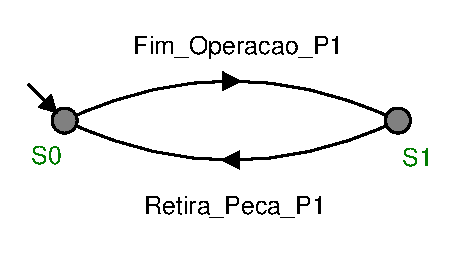
\includegraphics[width=\textwidth]{imagens/E4.eps}
      \caption{E4}
      \label{fig:e4}
  \end{subfigure}
  \hfill
  \begin{subfigure}[b]{0.45\textwidth}
      \centering
      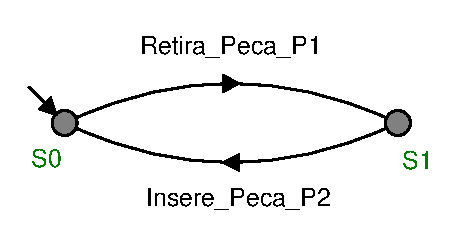
\includegraphics[width=\textwidth]{imagens/E5.eps}
      \caption{E5}
      \label{fig:e5}
  \end{subfigure}
  \caption{Especificações 4 e 5}
  \label{fig:e45}
\end{figure}

A especificação apresentada na Figura \ref{fig:e6} permite que a Prensa 2 inicie a operação após o Robô 2 finalizar a inserção e estar em posição segura.
Já a especificação apresentada na \ref{fig:e7} é o modelo para overflow da Prensa 2 e libera uma nova inserção após a retirada da peça pelo Robô 3.

\begin{figure}[H]%
  \centering
  \begin{subfigure}{0.45\textwidth}
      \centering
      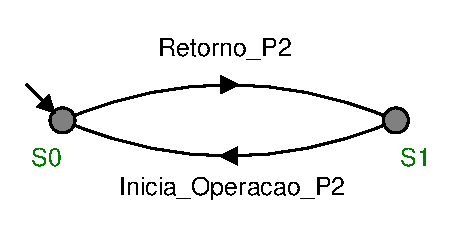
\includegraphics[width=\textwidth]{imagens/E6.eps}
      \caption{E6}
      \label{fig:e6}
  \end{subfigure}
  \hfill
  \begin{subfigure}{0.45\textwidth}
      \centering
      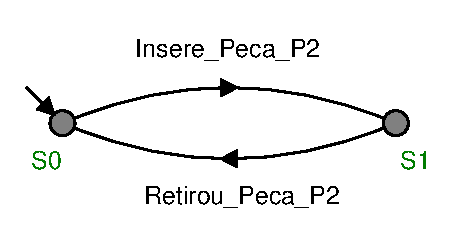
\includegraphics[width=\textwidth]{imagens/E7.eps}
      \caption{E7}
      \label{fig:e7}
  \end{subfigure}
  \caption{Especificações 6 e 7}
  \label{fig:e67}
\end{figure}

A especificação apresentada na Figura \ref{fig:e8} limita o Robô 3 a retirar peça da Prensa 2 após o final da operação.
Já a especificação apresentada na \ref{fig:e9} limita o Robô 3 a iniciar o processo de inserção na Prensa 3 após ter peça presente na garra..

\begin{figure}[H]%
  \centering
  \begin{subfigure}{0.45\textwidth}
      \centering
      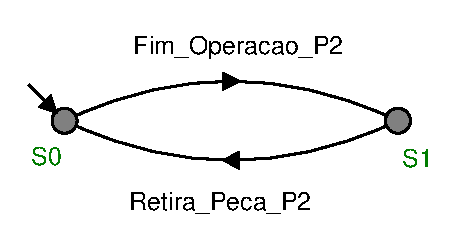
\includegraphics[width=\textwidth]{imagens/E8.eps}
      \caption{E8}
      \label{fig:e8}
  \end{subfigure}
  \hfill
  \begin{subfigure}{0.45\textwidth}
      \centering
      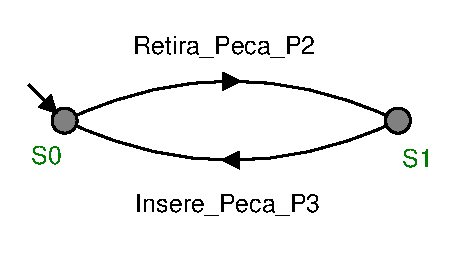
\includegraphics[width=\textwidth]{imagens/E9.eps}
      \caption{E9}
      \label{fig:e9}
  \end{subfigure}
  \caption{Especificações 8 e 9}
  \label{fig:e89}
\end{figure}

A especificação apresentada na Figura \ref{fig:e10} permite que a Prensa 3 inicie a operação após o Robô 3 finalizar a inserção e estar em posição segura.
Já a especificação apresentada na \ref{fig:e11} é o modelo para overflow da Prensa 3 e libera uma nova inserção após a retirada da peça pelo Robô 4.

\begin{figure}[H]%
  \centering
  \begin{subfigure}{0.45\textwidth}
      \centering
      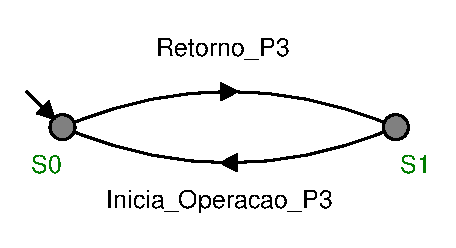
\includegraphics[width=\textwidth]{imagens/E10.eps}
      \caption{E10}
      \label{fig:e10}
  \end{subfigure}
  \hfill
  \begin{subfigure}{0.45\textwidth}
      \centering
      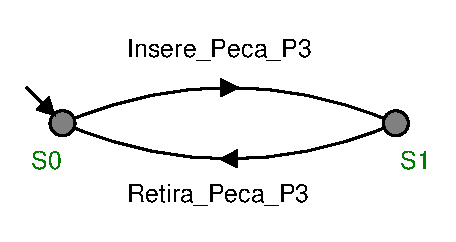
\includegraphics[width=\textwidth]{imagens/E11.eps}
      \caption{E11}
      \label{fig:e11}
  \end{subfigure}
  \caption{Especificações 10 e 11}
  \label{fig:e1011}
\end{figure}

A especificação apresentada na Figura \ref{fig:e12} limita o Robô 4 a retirar peça da Prensa 3 após o final da operação.
Já a especificação apresentada na \ref{fig:e13} limita o Robô 4 a iniciar o processo de entrega para Robô 5 após ter peça presente na garra.

\begin{figure}[H]%
  \centering
  \begin{subfigure}{0.45\textwidth}
      \centering
      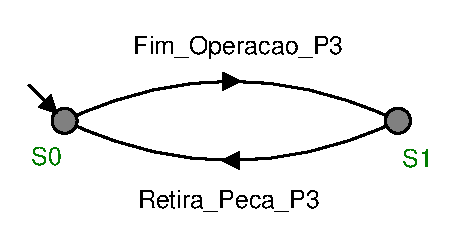
\includegraphics[width=\textwidth]{imagens/E12.eps}
      \caption{E12}
      \label{fig:e12}
  \end{subfigure}
  \hfill
  \begin{subfigure}{0.45\textwidth}
      \centering
      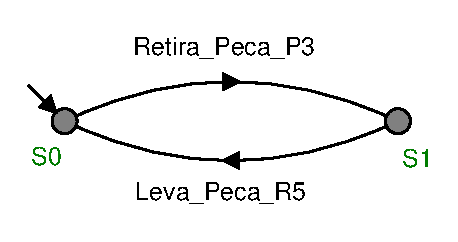
\includegraphics[width=\textwidth]{imagens/E13.eps}
      \caption{E13}
      \label{fig:e13}
  \end{subfigure}
  \caption{Especificações 12 e 13}
  \label{fig:e1213}
\end{figure}

A especificação apresentada na Figura \ref{fig:e14} permite que a Prensa 4 inicie a operação após o Robô 5 finalizar a inserção e estar em posição segura.
Já a especificação apresentada na \ref{fig:e15} limita o Robô 5 a retirar peça da Prensa 5 após o final da operação.

\begin{figure}[H]%
  \centering
  \begin{subfigure}{0.45\textwidth}
      \centering
      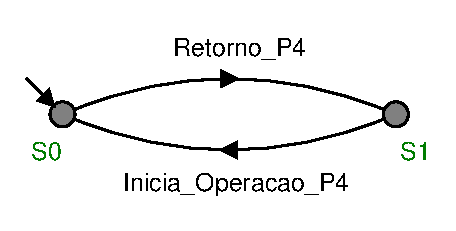
\includegraphics[width=\textwidth]{imagens/E14.eps}
      \caption{E14}
      \label{fig:e14}
  \end{subfigure}
  \hfill
  \begin{subfigure}{0.45\textwidth}
      \centering
      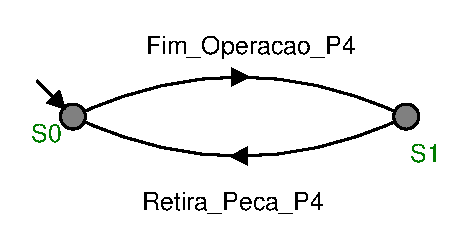
\includegraphics[width=\textwidth]{imagens/E15.eps}
      \caption{E15}
      \label{fig:e15}
  \end{subfigure}
  \caption{Especificações 14 e 15}
  \label{fig:e1415}
\end{figure}

A especificação apresentada na Figura \ref{fig:e16} força Robô 4 ao entregar uma peça aguarde o movimento do Robô 5 de buscar a peça.
Já a especificação apresentada na \ref{fig:e17} força o Robô 4 a aguardar posição segura do Robô 5 para retornar do movimento de entrega de peça.

\begin{figure}[H]%
  \centering
  \begin{subfigure}{0.45\textwidth}
      \centering
      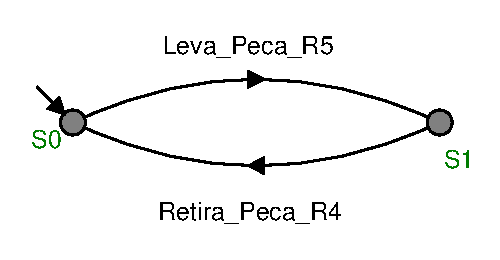
\includegraphics[width=\textwidth]{imagens/E16.eps}
      \caption{E16}
      \label{fig:e16}
  \end{subfigure}
  \hfill
  \begin{subfigure}{0.45\textwidth}
      \centering
      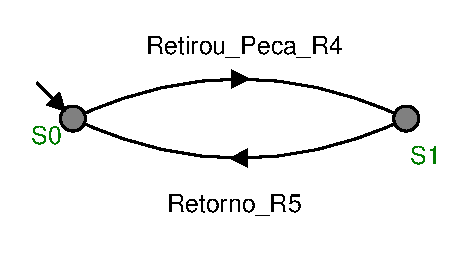
\includegraphics[width=\textwidth]{imagens/E17.eps}
      \caption{E17}
      \label{fig:e17}
  \end{subfigure}
  \caption{Especificações 16 e 17}
  \label{fig:e1617}
\end{figure}

A especificação apresentada na Figura \ref{fig:e18} limita o Robô 5 a iniciar o processo de inserção na Prensa 4 após ter peça presente na garra.
Já a especificação apresentada na \ref{fig:e19} permite que o Robô 5 pegue uma nova peça do Robô 4 após entregar a peça manufaturada na esteira.

\begin{figure}[H]%
  \centering
  \begin{subfigure}{0.45\textwidth}
      \centering
      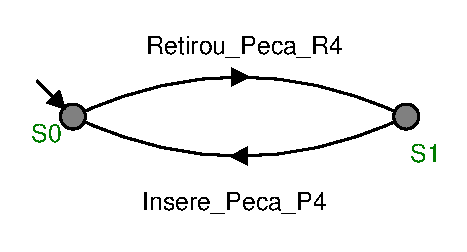
\includegraphics[width=\textwidth]{imagens/E18.eps}
      \caption{E18}
      \label{fig:e18}
  \end{subfigure}
  \hfill
  \begin{subfigure}{0.45\textwidth}
      \centering
      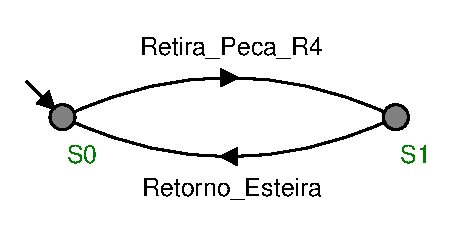
\includegraphics[width=\textwidth]{imagens/E19.eps}
      \caption{E19}
      \label{fig:e19}
  \end{subfigure}
  \caption{Especificações 18 e 19}
  \label{fig:e1819}
\end{figure}

\subsection{Solução modular de controle}
O software Supremica \cite{Supremica2020} disponibiliza funcionalidade para verificação da modularidade dos modelos desenvolvidos.
A Figura \ref{fig:modulare0} apresenta o resultado da análise da modularidade da especificação E0 com as plantas, podemos verificar que a especificação realiza controle de eventos sobre o Robô 1 e sobre Sensor Chapa sem ter dependencia com outras plantas.

\begin{figure}[H]%
  \centering
  \includegraphics[width=0.8\textwidth]{imagens/modular_E0.eps}
  \caption{Planta industrial}\label{fig:modulare0}
\end{figure}

O processo de verificação de modularidade foi executado para todas as especificações, a tabela \ref{tab:modulos} apresenta o resultado para cada especificação e as respectivas plantas com atuação.
Foi verificado que o número máximo de interações de uma especificações é com duas plantas.

\begin{table}[h]
\begin{center}
\begin{minipage}{0.5\textwidth}
\caption{Relações entre plantas e especificações}
\label{tab:modulos}
\begin{tabular}{@{}lll@{}}
  \toprule
  Especificação &  Planta 1 & Planta 2\\
  \midrule
  E0 & Sensor Chapa & Robô 1\\
  E1 & Robô 1 & \\
  E2 & Robô 1 & Prensa 1\\
  E3 & Robô 1 & Robô 2\\
  E4 & Robô 2 & Prensa 1\\
  E5 & Robô 2 & \\
  E6 & Robô 2 & Prensa 2\\
  E7 & Robô 2 & Robô 3\\
  E8 & Robô 3 & Prensa 2\\
  E9 & Robô 3 & \\
  E10 & Robô 3 & Prensa 3\\
  E11 & Robô 3 & Robô 4\\
  E12 & Robô 4 & Prensa 3\\
  E13 & Robô 4 & \\
  E14 & Robô 5 & Prensa 4\\
  E15 & Robô 5 & Prensa 4\\
  E16 & Robô 4 & Robo 5\\
  E17 & Robô 4 & Robo 5\\
  E18 & Robô 5 & \\
  E19 & Robô 5 & \\
  \botrule
\end{tabular}
\end{minipage}
\end{center}
\end{table}

A Tabela \ref{tab:supervisor} apresenta o número de estados, transições e eventos para cada supervisor modular e para o supervisor final.

\begin{table}[h]
\begin{center}
\begin{minipage}{0.5\textwidth}
\caption{Supervisores Modulares}
\label{tab:supervisor}
\begin{tabular}{@{}llll@{}}
  \toprule
  Supervisor & Estados & Eventos & Transições\\
  \midrule
  Sup 0 & 6 & 6 & 17\\
  Sup 1 & 6 & 6 & 10\\
  Sup 2 & 24 & 10 & 73\\
  Sup 3 & 32 & 12 & 120\\
  Sup 4 & 24 & 10 & 73\\
  Sup 5 & 6 & 6 & 10\\
  Sup 6 & 24 & 10 & 73\\
  Sup 7 & 32 & 12 & 120\\
  Sup 8 & 24 & 10 & 73\\
  Sup 9 & 6 & 6 & 10\\
  Sup 10 & 24 & 10 & 73\\
  Sup 11 & 32 & 12 & 120\\
  Sup 12 & 24 & 10 & 73\\
  Sup 13 & 6 & 6 & 10\\
  Sup 14 & 30 & 12 & 98\\
  Sup 15 & 30 & 12 & 98\\
  Sup 16 & 40 & 14 & 159\\
  Sup 17 & 40 & 14 & 159\\
  Sup 18 & 9 & 8 & 18\\
  Sup 19 & 9 & 8 & 18\\
  \midrule
  \textbf{Final} & & &\\
  \botrule
\end{tabular}
\end{minipage}
\end{center}
\end{table}

\bibliography{sn-bibliography}

\end{document}
